\documentclass[conference]{IEEEtran}
\usepackage{booktabs}
\usepackage{graphicx}
\usepackage{tikz}
\usetikzlibrary{arrows.meta,positioning}

\title{Clinical-Only Overall Survival Prediction in an MDA Head and Neck Cancer Cohort: An Exploratory Cox Model Study}
\author{\IEEEauthorblockN{Tharuniya Anpalakan}
\IEEEauthorblockA{Department of Applied Sciences\\
Northumbria University\\
Newcastle upon Tyne, United Kingdom\\
\texttt{w25070895@northumbria.ac.lk}}}

\begin{document}
\maketitle

\begin{abstract}This exploratory study describes a clinical-only Cox proportional hazards analysis of overall survival in an MDA clinical head and neck cancer dataset. The table contains 156 unique patient records, 43 recorded deaths, and 113 censored observations. A Cox model with age, sex, and encoded HPV status, using a penalizer of 1.0, achieved a saved mean five-fold cross-validated concordance index (C-index) of 0.615498 with random seed 42. HPV status was missing for 116 of 156 patients; the current dummy encoding does not distinguish missing HPV from the reference category. Candidate feature sets were compared using cross-validation, and the selected model has no independent external test or reported uncertainty interval. Separately, a 12-patient synthetic example demonstrates the mechanics of leave-one-centre-out evaluation; its scores are not clinical results. These findings describe an exploratory clinical baseline for overall survival and do not establish performance on unseen real centres or the value of imaging features.
\end{abstract}

\begin{IEEEkeywords}
overall survival, head and neck cancer, Cox proportional hazards, clinical prediction, cross-validation
\end{IEEEkeywords}

\section{Introduction}
This paper reports what the repository's completed analyses support: an exploratory clinical-only model for \emph{overall survival} and a separate synthetic example of a centre-held-out evaluation pipeline. Published work describes an MD Anderson head and neck squamous cell carcinoma (HNSCC) cohort archived by The Cancer Imaging Archive (TCIA) with clinical and survival information~\cite{grossberg2018}. The HECKTOR 2022 overview places MD Anderson data within the broader PET/CT and outcome-prediction challenge~\cite{andrearczyk2023hecktor}. These sources provide background context; they do not establish the derivation of the local CSV.

The contribution is a transparent account of the available cohort, implemented modelling steps, saved validation metric, and limitations. The repository protocol proposes recurrence-free survival and PET/CT radiomics comparisons, but those experiments were not completed. The synthetic example illustrates evaluation code only; it does not provide real multi-centre validation.

\section{Data and Methods}
\subsection{Real Clinical Table and Outcome}
The analysed local table is an MDA-labelled clinical dataset with 156 patient records and 84 variables. Published work describes an MD Anderson HNSCC cohort available through TCIA with clinical and survival data~\cite{grossberg2018}; however, the exact provenance and derivation of the local CSV were \emph{not independently re-verified} here. The analysis uses \texttt{Survival (months)} as duration and \texttt{Overall Survival Censor} as the event indicator. Its 43 values of 1 correspond to records labelled \texttt{Dead}; its 113 values of 0 correspond to records labelled \texttt{Alive}. The measured endpoint in this analysis is \emph{overall survival}, in months. Inclusion criteria beyond what the local table establishes remain unverified. No centre identifier or real centre-held-out test is used in the completed analysis.

\begin{table}[t]
\caption{Real Clinical Cohort and Analysis Variables}
\label{tab:cohort}
\centering
\footnotesize
\begin{tabular}{@{}p{0.57\columnwidth}p{0.32\columnwidth}@{}}
\toprule
Item & Value \\
\midrule
Unique patient records & 156 \\
Recorded deaths (event $=1$) & 43 \\
Censored observations (event $=0$) & 113 \\
Outcome & Overall survival, months \\
Model predictors & Age, sex, encoded HPV \\
HPV status recorded & 40/156 \\
\quad Positive; negative & 29; 11 \\
HPV status missing & 116/156 \\
\bottomrule
\end{tabular}
\end{table}

\subsection{Real-Data Modelling and Validation}
The notebook selects age, sex, HPV status, survival time, and event status. It applies \texttt{pandas.get\_dummies(..., drop\_first=True)} to sex and HPV status and then drops rows with missing values. Because the dummy \texttt{HPV status\_positive} is zero both for recorded HPV-negative entries and for missing HPV entries, this encoding \emph{does not distinguish missing HPV from the reference category}. All 156 rows remain in the resulting model table. The final model uses Cox proportional hazards methodology~\cite{cox1972} with a penalizer of 1.0.

The notebook evaluates prognostic discrimination using a concordance index~\cite{harrell1982} with five-fold cross-validation and seed 42. The saved result is the arithmetic mean of its five fold C-indices: \textbf{0.615498}. The repository does not save those five seeded fold scores separately, an uncertainty interval, or independent external-test predictions.

Exploratory candidate feature sets were compared using cross-validation. The selected age, sex, and HPV model must therefore be treated as exploratory: its reported cross-validation mean is not an independent confirmation of the choice. The notebook also calculates apparent C-indices on the data used to fit an age-only model and a larger multivariable model. These are labelled as training results in Table~\ref{tab:real-results}.

\subsection{Synthetic Centre-Aware Pipeline Demonstration}
A separate hand-entered example contains 12 patients assigned to synthetic centres A, B, and C, with four patients per centre. The demonstration holds out each centre in turn, learns HPV and T-stage missing-value replacements from the training portion, fits a Cox model with age, HPV-positive indicator, and T stage, and scores the held-out example patients. The pipeline uses a Cox penalizer of 0.1 for the reported centre-wise scores. These artificial records and scores are separate from the MDA clinical table and cannot assess real cross-centre generalization. Figure~\ref{fig:workflow} keeps the two analyses visually separate.

\begin{figure}[t]
\centering
\resizebox{\columnwidth}{!}{%
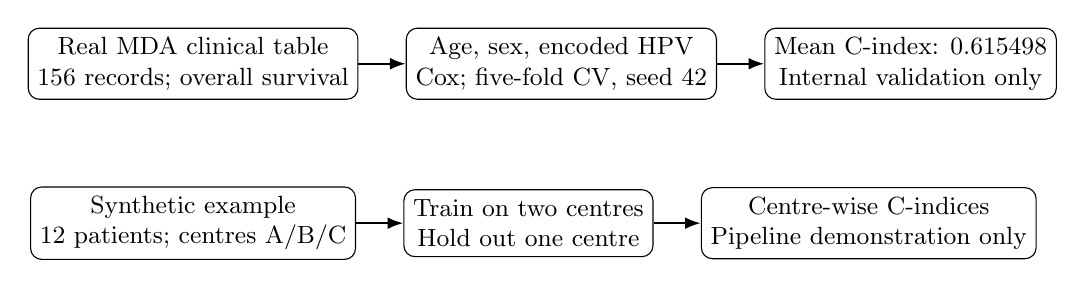
\begin{tikzpicture}[
  box/.style={draw, rounded corners, align=center, minimum width=3.1cm, minimum height=0.85cm, font=\small},
  arr/.style={-{Latex[length=2mm]}, thick},
  node distance=0.6cm
]
\node[box] (real1) {Real MDA clinical table\\156 records; overall survival};
\node[box, right=of real1] (real2) {Age, sex, encoded HPV\\Cox; five-fold CV, seed 42};
\node[box, right=of real2] (real3) {Mean C-index: 0.615498\\Internal validation only};
\draw[arr] (real1) -- (real2);
\draw[arr] (real2) -- (real3);
\node[box, below=1.1cm of real1] (syn1) {Synthetic example\\12 patients; centres A/B/C};
\node[box, right=of syn1] (syn2) {Train on two centres\\Hold out one centre};
\node[box, right=of syn2] (syn3) {Centre-wise C-indices\\Pipeline demonstration only};
\draw[arr] (syn1) -- (syn2);
\draw[arr] (syn2) -- (syn3);
\end{tikzpicture}%
}
\caption{Separate workflows for the real clinical overall-survival analysis and the 12-patient synthetic centre-aware pipeline demonstration. The lower branch is not real multi-centre validation.}
\label{fig:workflow}
\end{figure}

\section{Results}
\subsection{Real MDA Overall-Survival Analysis}
The saved final result is a \textbf{mean five-fold cross-validated C-index of 0.615498 (seed 42)} for the clinical-only Cox model. This is a discrimination estimate from internal cross-validation, not evidence of clinical utility or external-centre performance. The age-only and larger multivariable values in Table~\ref{tab:real-results} were measured on their training data; their differing feature sets and validation methods prevent a like-for-like performance comparison with the selected model.

\begin{table}[!htbp]
\caption{Real MDA Overall-Survival Model Results. Apparent Values Are Training C-Indices, Not Held-Out Estimates}
\label{tab:real-results}
\centering
\scriptsize
\begin{tabular}{@{}p{0.43\columnwidth}p{0.33\columnwidth}r@{}}
\toprule
Model and predictors & Evaluation & C-index \\
\midrule
Age-only Cox (age) & Apparent training & 0.568 \\
Larger multivariable Cox, penalizer 0.1 (age, sex, site, histology, grade, T, N, HPV status) & Apparent training & 0.760 \\
Selected clinical Cox, penalizer 1.0 (age, sex, encoded HPV status) & Mean five-fold cross-validation, seed 42 & \textbf{0.615498} \\
\bottomrule
\end{tabular}
\end{table}

The notebook also evaluated an age, sex, HPV status, and grade candidate using the same seeded five-fold approach. Its reported mean was approximately 0.563434. Because feature sets were compared on cross-validation results, neither that contrast nor the selected result constitutes independent model confirmation.

\subsection{Synthetic Pipeline Demonstration}
The synthetic centre-held-out scores in Table~\ref{tab:synthetic} are shown solely to document operation of the pipeline. Each held-out group has four example patients. The mean of the three reported centre C-indices is 0.244333; it is \emph{not} an estimate of real multi-centre performance. The synthetic notebook also records convergence warnings during unpenalized exploratory fits, consistent with the very small example size.

\begin{table}[!htbp]
\caption{Synthetic Centre-Aware Pipeline Demonstration Only}
\label{tab:synthetic}
\centering
\begin{tabular}{@{}lcc@{}}
\toprule
Synthetic held-out centre & Example patients & C-index \\
\midrule
A & 4 & 0.200 \\
B & 4 & 0.333 \\
C & 4 & 0.200 \\
\bottomrule
\end{tabular}
\end{table}

\section{Discussion}
The real analysis provides a recorded internal cross-validation result for a limited clinical predictor set. Its mean C-index of 0.615498 should be interpreted cautiously because HPV status is mostly missing and encoded with the reference category, candidate feature sets were compared using cross-validation, and there is no independent external test. The apparent training values in Table~\ref{tab:real-results} cannot be read as held-out results.

The synthetic demonstration verifies that centre splitting, training-only missing-value replacement, model fitting, and held-out scoring can be executed on the example data. Its numerical scores are not evidence about patient prognosis or robustness across real centres. No PET/CT image features, radiomics, multimodal model, or recurrence-free-survival experiment is reported here.

\section{Limitations and Future Work}
The completed real experiment addresses overall survival only. The local table does not support a completed real centre-held-out experiment, and the repository has no independent external test set for the selected model. The final C-index has no reported uncertainty interval, and only one seeded five-fold split is saved. Candidate feature-set comparison used cross-validation; the selected model is exploratory and not independently confirmed. The notebook does not report a final-model proportional-hazards diagnostic or calibration assessment.

HPV status is missing for 116/156 patients. The current encoding maps missing HPV and the recorded reference category to the same dummy value, so the fitted HPV coefficient and model performance require caution. A future analysis should explicitly handle missingness within training folds, prespecify the model-selection process, and report uncertainty. Real centre-aware validation would require identified patients from multiple real centres and a held-out-centre design. PET/CT radiomics and recurrence-free-survival studies remain future work, subject to suitable data and an appropriate protocol.

\section{Conclusion}
The completed repository work supports an exploratory, clinical-only overall-survival Cox analysis in 156 records from the analysed MDA clinical dataset, with a saved mean five-fold cross-validated C-index of \textbf{0.615498} at seed \textbf{42}. The separate 12-patient synthetic example demonstrates centre-aware pipeline mechanics only. Neither result establishes real multi-centre generalization, imaging benefit, or clinical utility.

\bibliographystyle{IEEEtran}
\bibliography{references}
\end{document}
